\documentclass[12pt,twoside]{article}

\usepackage[ampersand]{easylist}
\usepackage[finnish]{babel}
\usepackage[utf8]{inputenc}
\usepackage{sectsty}
\usepackage{titlesec}
\usepackage{enumitem}
\usepackage{fancyhdr}
\usepackage{graphicx}
\usepackage{hyperref}


\usepackage{sidecap}
\usepackage[font=sf]{caption}
\sidecaptionvpos{figure}{t}

\usepackage{geometry}
 \geometry{
 a4paper,
 total={170mm,240mm},
 left=20mm,
 top=25mm,
 footskip=18mm
 }
 
\fontfamily{lmss}\selectfont 
\pagestyle{fancy}
\fancyhf{}
\renewcommand{\headrulewidth}{0pt}
\fancyhead[LE,RO]{\thepage}
\lfoot{\fontfamily{lmss}\selectfont Creative Commons BY-NC-SA}
\rfoot{\fontfamily{lmss}\selectfont Alkuperäinen tekijä (2016) Anni Järvenpää}

\newenvironment{vaihetaso1}{%
    \LARGE
    \itemize
}{%
    \enditemize
}
\newenvironment{vaihetaso2}{%
    \Large
    \itemize
}{%
    \enditemize
}
\newenvironment{vaihetaso3}{%
    \large
    \itemize
}{%
    \enditemize
}

\setitemize{topsep=0pt,parsep=10pt}

\newcommand{\laatikkoyksi}{\raisebox{0ex}{\framebox(15,15)}}
\renewcommand{\labelitemi}{\laatikkoyksi}
\newcommand{\laatikkokaksi}{\raisebox{0ex}{\framebox(12,12)}}
\renewcommand{\labelitemii}{\laatikkokaksi}
\newcommand{\laatikkokolme}{\raisebox{0ex}{\framebox(10,10)}}
\renewcommand{\labelitemiii}{\laatikkokolme}

\sectionfont{\fontfamily{lmss}\fontsize{35}{35}\selectfont}
\subsectionfont{\fontsize{25}{40}\fontfamily{lmss}\selectfont}
\titlespacing*{\section}{3em}{0em}{2em}
\titlespacing*{\subsection}{1.5em}{1em}{1em}


\begin{document}
\fontfamily{lmss}\selectfont
\section*{Pelin nimi}

\begin{SCfigure}[][h]
  \centering
  \captionsetup{labelformat=empty}
  \caption{Lyhyt kuvaus pelistä, mitä siinä tehdään ja mihin pyritään. \href{https://google.fi}{Linkki mallipeliin}, tekijän nimi ja pelin nimi näkyviin että tulosteenkin perusteella on mahdollista löytää.}
  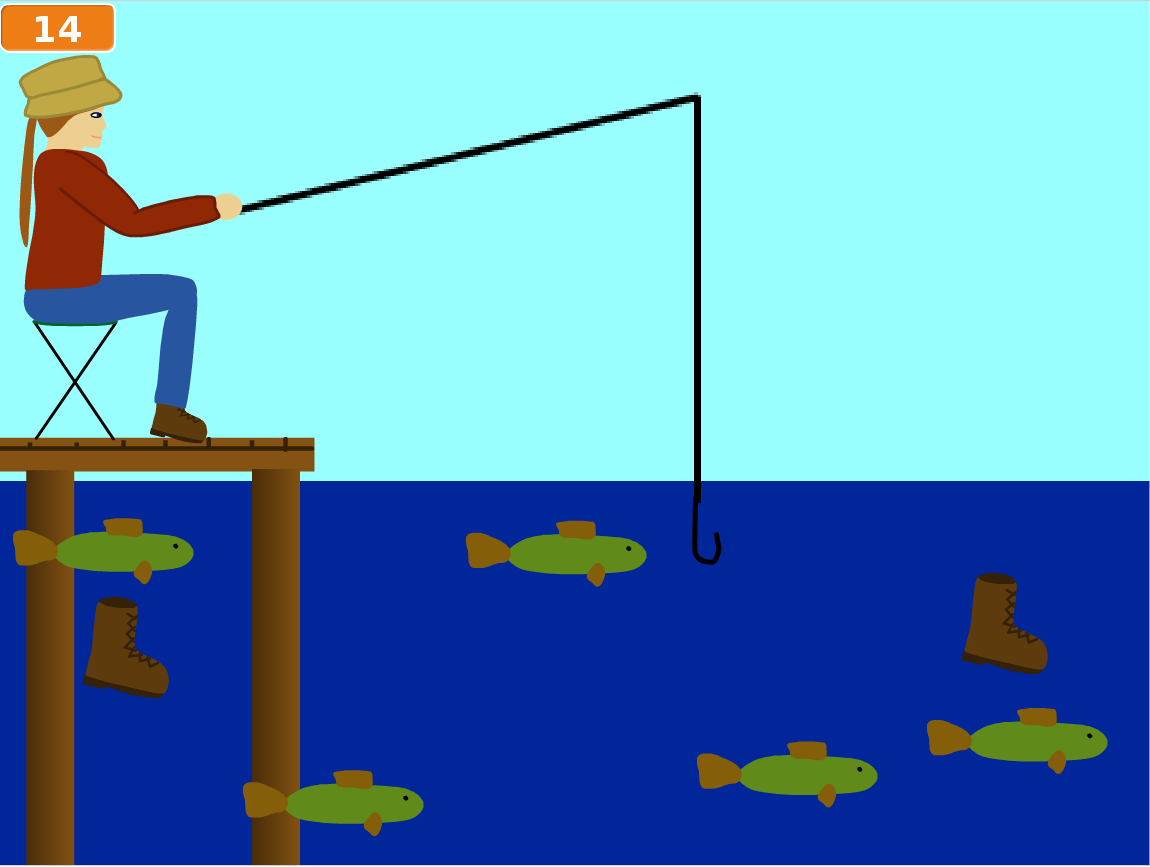
\includegraphics[width=0.7\textwidth]{kuvat/esimerkki.png}
\end{SCfigure}

\begin{vaihetaso1}
	\item Ensimmäinen ohje
	\begin{vaihetaso2}
		\item Yhden lauseen kuvaus
		\item Tällä on alakohta
		\begin{vaihetaso3}
			\item Turhan syvä alakohta
		\end{vaihetaso3}
		\item Pitkähkö kuvaus siitä, mitä nyt pitää tehdä. Monimutkaiset ohjelmat ovat monimutkaisia. Onneksi lapset ovat fiksuja.
	\end{vaihetaso2}
	\item Toinen vaihe
	\begin{vaihetaso2}
		\item Laatikoita pukkaa
		\item Tällä on alakohta
		\item Lorem ipsum
	\end{vaihetaso2}
	\item Kolmas vaihe
	\item Neljäs vaihe
\end{vaihetaso1}

\subsection*{Väliotsikko}

\begin{vaihetaso1}
	\item Ensimmäinen ohje
	\begin{vaihetaso2}
		\item Yhden lauseen kuvaus
		\item Tällä on alakohta
		\begin{vaihetaso3}
			\item Turhan syvä alakohta
		\end{vaihetaso3}
		\item Pitkähkö kuvaus siitä, mitä nyt pitää tehdä. Monimutkaiset ohjelmat ovat monimutkaisia. Onneksi lapset ovat fiksuja.
	\end{vaihetaso2}
	\item Toinen vaihe
	\item Vielä yksi
	\begin{vaihetaso2}
		\item Laatikoita pukkaa
		\item Tällä on alakohta
		\item Lorem ipsum
	\end{vaihetaso2}
	\item Kolmas vaihe
	\item Neljäs vaihe
\end{vaihetaso1}

% halutessaan voi alemman %-merkin poistamalla pakottaa laajennusideat omalle sivulleen
%\newpage
\subsection*{Laajennusideoita}
\begin{itemize}
	\item[-] Muita hauskoja juttuja, joita peliin voisi halutessaan toteuttaa
	\item[-] Voi olla myös alakohtia:
	\begin{itemize}
		\item[-] Ensimmäinen alakohta
		\item[-] Toinen alakohta
		\item[-] Kolmas alakohta
	\end{itemize} 
	\item[-] Vielä tavallinen idea perään
\end{itemize}

\end{document}